\chapter{Experiments and Results}\label{chapter:results}
\section{Experiments}\label{section:exp}
For the experiments, we used, for the first 100K training episodes of the three techniques, Helios2013's goalie and Helios2013's offensive and for 10K we changed the goalie to RoboCIn2019's. We used \cite{dqn}'s technique to stack 32 states, therefore a state of shape [32x1x16]. The Networks' and memory's parameters is in Figure \ref{fig:hyperparams}. For DQN and DDQN we used the $\epsilon$-greedy technique with $\epsilon$'s maximum at 1.0 and minimum at 0.01. For DDPG we added a noise of 0.1 in the action. The full code is available in \url{https://github.com/goncamateus/graduationMgm}.

The Neural Network's topology were (all using Rectified Linear Unit activation function \cite{relu}):
\begin{itemize}
    \item Deep Q Networks: 512:128:256:4.
    \item Duelling Double Deep Q Networks: 
    
    Advantage - [512:128:128:4]; Value - [512:128:128:1].
    \item Deep Deterministic Policy Gradient: 
    
    Actor - [512:256:128] with output of shape [4x1]; Critic - [512:256:128:1].
\end{itemize}


\begin{figure}
    \centering
    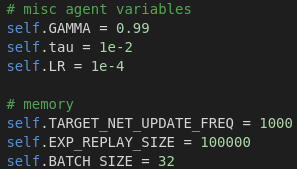
\includegraphics[scale=0.6]{images/hyperparams.png}
    \caption{Neural Networks' and Memory's parameters.}
    \label{fig:hyperparams}
\end{figure}

\section{Results}
In this section we show the graphs and tables of training and tests. As said in Section \ref{section:exp}, the training was 100K episodes with Helios2013's goalie and 10K with RoboCIn2019's goalie. The whole training against Helios2013's attacker.
\subsection{Training}
During the training we could see some interesting behaviours of each learning algorithm. The DQN agent turned out to be the most aggressive agent. Before episode 10K, it started to chase the attacker due to Intercept action. As there is no fault in our domain, the Network found this strategy but it is not the best thing to be done during a real game. Figure \ref{fig:dqnres} shows it's performance with rewards.
\begin{figure}[H]
    \centering
    \subfloat{{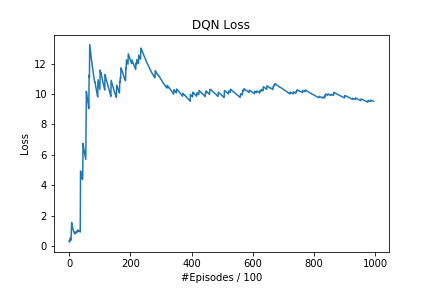
\includegraphics[scale=0.45]{images/dqn_loss.png}}}%
    \qquad
    \subfloat{{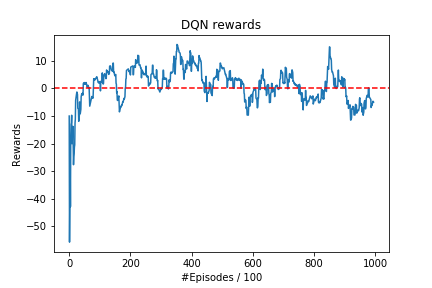
\includegraphics[scale=0.45]{images/dqn_rewards.png}}}%
    \qquad
        \caption{Deep Q Network results. Loss convergence and Rewards in function of number of episodes.}
    \label{fig:dqnres}
\end{figure}

The DDPG agent found a policy very similar to RoboCIn2019's defender but a bit more aggressive. The agent blocks the shoot of the attacker most of time but intercept in the right gap of the attacker. Sometimes the episode takes too long due to the attacker's incapability to decide what to do, that would lead to a fault in real game and the defender would win the ball. Figure \ref{fig:ddpgres} shows the performance of the agent. As we can  see in the Actor Loss, sometime before the episode 20K it found that policy and converged to it.

\begin{figure}[H]
    \centering
    \subfloat{{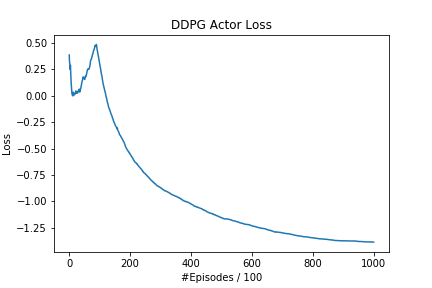
\includegraphics[scale=0.45]{images/ddpg_actor_loss.png}}}%
    \qquad
    \subfloat{{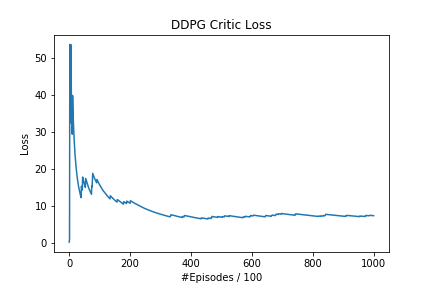
\includegraphics[scale=0.45]{images/ddpg_critic_loss.png}}}%
    \qquad
    \subfloat{{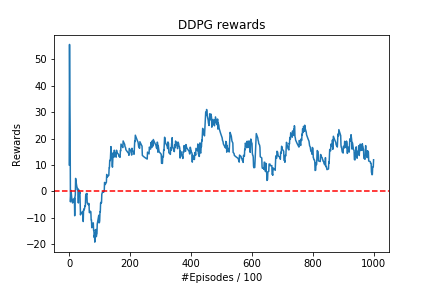
\includegraphics[scale=0.6]{images/ddpg_rewards.png}}}%
    \qquad
    \caption{Deep Deterministic Policy Gradient results. Loss convergence of Actor and Critic networks and Rewards in function of number of episodes.}
    \label{fig:ddpgres}
\end{figure}

The DDQN agent took an intermediate behaviour. Sometimes it acted as DQN's agent but most of time it acted just like DDPG's. The episodes that it acted too aggressive, the attacker shoots to the goal and scores, most of time. Figure \ref{fig:ddqnres} shows the performance of the agent.

\begin{figure}[H]
    \centering
    \subfloat{{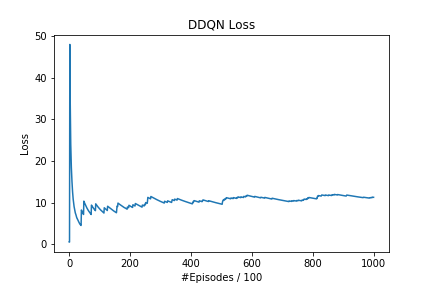
\includegraphics[scale=0.45]{images/ddqn_loss.png}}}%
    \qquad
    \subfloat{{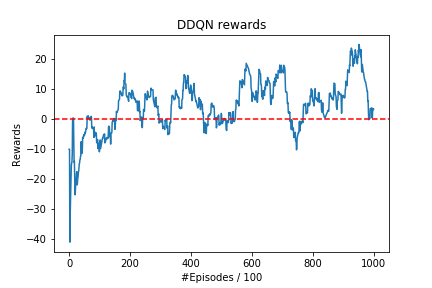
\includegraphics[scale=0.45]{images/ddqn_rewards.png}}}%
    \qquad
        \caption{Duelling Double Deep Q Network results. Loss convergence and Rewards in function of number of episodes.}
    \label{fig:ddqnres}
\end{figure}




\subsection{Tests}
To test, we wanted to compare with the Helios2013 and RoboCIn2019. Helios2013 was chosen because HFO already had support for the team. RoboCIn2019 was chosen because we want to put the best agent in the team. We tested with both attackers and both goalies for 3000 episodes each combination. Table \ref{tab:result_base_line} shows the baseline with Helios2013's and RoboCIn2019's agents. Tables \ref{tab:helios_result} and \ref{tab:rc_result} show the results of the DRL agents with the cooperating with the deterministic goalies against each attacker.

\begin{table}[H]
\begin{center}
\begin{tabular}{|c|c|c|}
\hline

                   & Helios2013 & RoboCIn2019 \\ \hline
Helios2013         & 77,5\%     & 77.4\%      \\ \hline
RoboCIn2019        & 71\%       & 53.3\%      \\ \hline
    \end{tabular}
\end{center}
\caption{Result baseline. Rows are the defenders and Columns are the attackers of each original team. Percentage of successful defenses for 3000 episodes.}
\label{tab:result_base_line}
\end{table}

\begin{table}[H]
\begin{center}
\begin{tabular}{|c|c|c|}
\hline
                   & Helios2013 & RoboCIn2019 \\ \hline
DQN 110k training  & 63\%     & 76.2\%        \\ \hline
DDQN 110k training & 75.1\%       & 72.4\%      \\ \hline
DDPG 110k training & 82.1\%     & 95\%      \\ \hline
\end{tabular}
\end{center}
\caption{Tests for 3000 episodes. Rows are the DRL defenders with Helios2013's goalie and Columns are the attackers. Percentage of successful defenses for 3000 episodes.}
\label{tab:helios_result}
\end{table}


\begin{table}[H]
\begin{center}
\begin{tabular}{|c|c|c|}
\hline
                   & Helios2013 & RoboCIn2019 \\ \hline
DQN 110k training  & 51.3\%     & 64.2\%        \\ \hline
DDQN 110k training & 62.9\%     & 83.6\%      \\ \hline
DDPG 110k training & 70\%     & 86.7\%      \\ \hline
\end{tabular}
\end{center}
\caption{Tests for 3000 episodes. Rows are the DRL defenders with RoboCIn2019's goalie and Columns are the attackers. Percentage of successful defenses for 3000 episodes.}
\label{tab:rc_result}
\end{table}